\documentclass[11pt, oneside, a4paper]{article}
\usepackage[utf8x]{inputenc}
\usepackage[serbianc]{babel}
\usepackage{tikz}
\usepackage{forest}
\usepackage{epigraph}
\usepackage{amssymb}
\usepackage{amsmath}
\usepackage[language=english]{biblatex}
\usepackage{kbordermatrix}
\usepackage[bottom]{footmisc}
\usepackage[export]{adjustbox}
\usepackage{geometry}
\usetikzlibrary{arrows, positioning,chains,fit,shapes, calc, topaths, arrows.meta, automata, positioning, graphs, graphs.standard}



\tikzset{
  treenode/.style = {align=center, inner sep=0pt, text centered,
    font=\sffamily},
  arn_n/.style = {treenode, circle, white, font=\sffamily\bfseries, draw=black,
    fill=black, text width=2em},% arbre rouge noir, noeud noir
  arn_r/.style = {treenode, circle, white, draw=red, fill = red, 
    text width=2em, very thick},% arbre rouge noir, noeud rouge
  arn_x/.style = {treenode, circle, white, font=\sffamily\bfseries, draw=black,
    fill=black, text width=2em}% arbre rouge noir, nil
}


\newcount\mycount

\begin{document}

\clearpage
\newgeometry{bottom=1cm, left=3cm,right=3cm}

\begin{center}
    {\huge Математичка гимназија}
\end{center}
\vspace{0.35\textheight}
\begin{center}\
    {\huge \textbf{МАТУРСКИ РАД\\}}
    {\huge Основни појмови и алгоритми из области \\ теорије графова}
\end{center}
\vspace{0.30\textheight}
\begin{flushleft}
\textbf{Ментор}: Станка Матковић \hfill
\textbf{Ученик}: Вељко Селаковић \\ \textbf{Предмет}: Програмирање \\
и програмски језици
\end{flushleft}
\vspace{0.05\textheight}
\begin{center}
    Београд, Јун 2019.
\end{center}
\thispagestyle{empty}

\restoregeometry



\newpage

\tableofcontents
\newpage
\section{Увод}
Један од највећих умова света, \textbf{Леонард Ојлер}, је 1752. године написао рад \glqq Седам мостова Кенингсберга\grqq, на који данас гледамо као на сам почетак теорије графова. Сама структура графа врло је блиска реалном свету, и као таква, изузетно је применљива у истом. Теорија графова данас је укорењена у много различитих области наших живота, од којих су неке круцијалне за нормално функционисање друштва. \par
Циљ овог рада јесте приближавање основних појмова везаних за графове читаоцу, као и алгоритме који се над њима врше. У првом делу рада упознајемо се са основним појмовима и некима од небројено много врста графова. Други део показује како алгоритми које вршимо функционишу, и колико су заиста битни за данашње информационо доба. На самом крају налазе се две од најпознатијијх теорема и проблема везаних за графове: \textit{Теорема о четири боје} и \textit{Проблем путујућег трговца}. Ова два проблема и њихова историја врло ефективно показују како и зашто се теорија графова развијала током година.


\newpage
\section{Граф}
Постоји много различитх дефиниција графа, а једна од најчешћих и најбазичнијих јесте: \glqq Граф је уређени пар $G=(V, E)$ којег чине скуп чворова \textbf{V} i скуп веа између тих чворова, \textbf{E}. Основна и најбитнија подела графа јесте на усмерене и неусмерене.
\subsection{Неусмерени (\textit{undirected}) граф}
Неусмерени графови су најбазичнија верзија структуре података која испуњава све дате услове да би била граф. Састоји се од чворова од којих су неки повезани ивицама. Све ивице су бидирекционе, што значи да ако имамо два чвора повезана ивицама можемо доћи из првог у други, и обратно.
\subsection{Усмерени (\textit{directed}) граф}
Код усмерених графова грана може имати задат смер. Ако имамо повезане чворове А и Б, и задату ивицу А $\rightarrow$ Б, из чвора А можемо доћи у чвор Б, али не и из Б у А.\par Добар пример усмерених графова био би градски саобораћај. Ако посматрамо раскрснице као чворове, једносмерне улице би биле усмерене, а двосмерне улице неусмерене ивице.
\subsection{Тежински (\textit{weighted}) граф}
Тежински графови имају задату вредност сваке ивице. Најчешће се користе за репрезентацију тачака на мапи и њихових удаљености (погледати \textit{проблем путујућег трговца}) или људског генома у генетичким прорачунима. Тежински граф чије све ивице имају вредност 0 је обичан, нетежински граф.
\begin{figure}[ht]
    \centering
    \begin{tikzpicture}[
    > = stealth, % arrow head style
    shorten > = 1pt, % don't touch arrow head to node
    auto,
    node distance = 3cm, % distance between nodes
    semithick % line style
    ]

    \tikzset{every state}=[
    draw = black,
    thick,
    fill = white,
    minimum size = 1mm
    ]

     \node[state] (y1) {$1$};
    \node[state] (x1) [above=of y1]{$3$};
    \node[state] (x2) [left=of x1] {$4$};
    \node[state] (x3) [right=of x1] {$5$};
    \node[state] (y3) [below=of x3] {$2$};


    \path[->] (x1) edge[red]  node[pos=0.25, above left] {5} (y1);
    \path[->] (x2) edge  node[] {4} (x1);
    \path[->] (x3) edge  node[] {3} (y3);
    \path[->] (y3) edge node[] {11} (x2);
    \path[->] (y1) edge node[] {10} (x3);

    \end{tikzpicture}
    \caption{Тежински граф}
    \label{fig:my_label}
\end{figure}

\subsection{Повезани (\textit{connected}) граф}
Повезаним графом називамо сваки граф чији су сви чворови повезани, односно постоји рута између сваког пара чворова. У случају да је граф усмерен, он може бити повезан, неповезан или слабо повезан. Ако заменимо све ивице неког усмереног графа неусмереним и добијемо повезани граф, тај граф називамо слабо повезаним. 
\subsection{Комплетни граф}
Комплетан граф је онај граф чији је сваки чвор повезан са свим осталим чворовима.
\begin{figure}[h]
    \centering
    \begin{tikzpicture}
        \graph { subgraph K_n [n=8,clockwise,radius=2cm] };
    \end{tikzpicture}

    \caption{Комплетан граф}
    \label{fig:my_label}
\end{figure}
\subsection{Бипартидни (\textit{bipartite}) граф}
Бипартидни граф је граф чије чворове можемо поделити у два дисјунктна скупа \textbf{U} и \textbf{V} тако да свака ивица повезује чвор из скупа \textbf{U} са чвором из скупа \textbf{V}. Ако је број елемената у оба скупа исти, тада је граф \textit{Балансирани бипартидни граф}. Ова врста графова има велику примену у теорији кодирања, углавном за декодирање порука.

\definecolor{myblue}{RGB}{64, 0, 255}
\definecolor{myorange}{RGB}{227, 66, 52}
\begin{figure}[h]
    \begin{minipage}{0.5\textwidth}
        \centering
    
        \begin{tikzpicture}
    
        \def \n {7}
        \def \radius {3cm}
        \def \margin {8} % margin in angles, depends on the radius
        
        \foreach \s in {1,...,\n}
        {
          \node[draw, circle] at ({360/\n * (\s - 1)}:\radius) {$\s$};
          \draw[->, >=latex] ({360/\n * (\s - 1)+\margin}:\radius) 
            arc ({360/\n * (\s - 1)+\margin}:{360/\n * (\s)-\margin}:\radius);
        }
        \end{tikzpicture}
    
        \caption{Циклични граф}
        \label{fig:my_label}
    \end{minipage}
    \begin{minipage}{0.5\textwidth}
    \centering
    \begin{tikzpicture}[thick,
      every node/.style={draw,circle},
      fsnode/.style={fill=myblue},
      ssnode/.style={fill=myorange},
      every fit/.style={ellipse,draw,inner sep=-2pt,text width=2cm},
      -,shorten >= 3pt,shorten <= 3pt
    ]
    
    % the vertices of U
    \begin{scope}[start chain=going below,node distance=7mm]
    \foreach \i in {1,2,...,5}
      \node[fsnode,on chain] (f\i) [] {};
    \end{scope}
    
    % the vertices of V
    \begin{scope}[xshift=4cm,yshift=-0.5cm,start chain=going below,node distance=7mm]
    \foreach \i in {6,7,...,9}
      \node[ssnode,on chain] (s\i) [] {};
    \end{scope}
    
    % the set U
    \node [myblue,fit=(f1) (f5),label=above:$U$] {};
    % the set V
    \node [myorange,fit=(s6) (s9),label=above:$V$] {};
    
    % the edges
    \draw (f1) -- (s6);
    \draw (s6) -- (f2);
    \draw (f2) -- (s7);
    \draw (s7) -- (f3);
    \draw (s8) -- (f3);
    \draw (f3) -- (s9);
    \draw (s9) -- (f5);
    \draw (f5) -- (s6);
    \end{tikzpicture}
    \caption{Бипардтидни граф}
    \end{minipage}
\end{figure}

\subsection{Циклични (\textit{cycle}) граф}
\textbf{Циклус} је део графа где проласком кроз њега можемо два пута приступити истом чвору. \par
\textbf{Степен} чвора је број суседа тог чвора. \par
Цикличним графом називамо граф кoјег чини само један циклус. Последице тога јесу да сваки циклични граф \textit{$G_n$} има \textbf{n} чворова и \textbf{n} ивица, као и да сваки чвор има степен 2. Сви циклични графови чији је број елемената паран су бипартидни графови. 



\subsection{Стабло (\textit{tree})}
Стабла су специјални подслучај графа где постоји \emph{тачно} једна путања између свака два чвора. Последица тога је да стабло увек мора да има $n-1$ грана на \textit{n} чворова. Код стабала постоји посебан начин означавања разних чворова. \par 
\textbf{Корен} стабла је чвор који није подчвор ниједног чвора у стаблу. \par
\textbf{Лист} је чвор који нема ни један подчвор.\par
\textbf{Родитељ} неког чвора је чвор који показује на њега. \par
\textbf{Подчвор} неког чвора \textbf{v} називамо \textbf{дететом} чвора \textbf{v}. \par
\textbf{Шумом} називамо скуп дисјунктних стабала који заједно представљају један \textit{неповезани} граф. По својој природи, свако стабло је \textit{бипартидни граф}. \par
Алгоритми које најчешће везујемо за стабла јесу \textit{Претрага у ширину} и \textit{Претрага у дубину}, јер су стабла идеална структура за схватање начина функционисања истих. 
\subsubsection*{Бинарно стабло}
Код бинарних стабала, сваки чвор може имати највише два потомка.
\subsubsection*{Црно-црвено стабло}
Црно-црвено стабло је подврста бинарних стабала која је самобалансирајућа. Сваки чвор има додатни бит који можемо тумачити као боју (црну или црвену). Ако потомак не постоји, одговарајући чвор обележавамо \textbf{NIL}, и посматрамо га као лист. Свако ЦЦ стабло мора испунити пет услова:
\begin{enumerate}
\item Сваки чвор је или црн или црвен.
\item Корен је црн.
\item Сви \textbf{NIL} чворови су црни.
\item Ако је чвор црвен, тада су његова деца црна.
\item Број црних чворова на сваком путу од једног чвора стабла до њему припадајућих листова је једнак.
\end{enumerate}
\begin{figure}[h]
    \centering


\begin{tikzpicture}[-,>=stealth',level/.style={sibling distance = 6cm/#1,
  level distance = 1.5cm}] 
\node [arn_n] {33}
    child{ node [arn_r] {15} 
            child{ node [arn_n] {10} 
            	child{ node [arn_r] {5} edge from parent node[above left]
                         {}} %for a named pointer
							child{ node [arn_x] {NIL}}
            }
            child{ node [arn_n] {20}
							child{ node [arn_r] {18}}
							child{ node [arn_x] {NIL}}
            }                            
    }
    child{ node [arn_r] {47}
            child{ node [arn_n] {38} 
							child{ node [arn_r] {36}}
							child{ node [arn_r] {39}}
            }
            child{ node [arn_n] {51}
							child{ node [arn_r] {49}}
							child{ node [arn_x] {NIL}}
            }
		}
; 
\end{tikzpicture}
\caption{Црно-црвено стабло}
\end{figure}
\subsubsection*{Дигитално стабло (\textit{Трие})}
Трие, или \textit{префиксно стабло} је структура података која се користи за ефикасно чување и претрагу стрингова. Код овог стабла, ниједан чвор не чува кључ који њему одговара, већ га сама његова позиција у стаблу одређује. Најчешћа примена дигиталног стабла јесте предикција текста, попут оне на мобилним уређајима. Осим тога, може да се користи и као речник. 
\begin{figure}[h]
    \centering
    \scalebox{0.6}{\begin{forest}
    for tree={
      circle,
      black,
      draw,
      fill=black,
    }
      [{}
        [{}, edge label={node [midway, above left] {О}}
          [{}, edge label={node [midway, right] {Л}}
            [{}, edge label={node [midway, right] {У}}
              [,phantom]
              [{}, edge label={node [midway, left] {Ј}}
                [{}, edge label={node [midway, left] {А}}, label=below:Олуја
                ]
                [,phantom]
              ]
              [{}, edge label={node [midway, right] {К}}, label=below:Олук
              ]
              [,phantom]
            ]
            [,phantom]
          ]
          [,phantom]
        ]
        [{}, edge label={node [midway, right] {К}}
          [{}, edge label={node [midway, right] {О}}
            [{}, edge label={node [midway, right] {Л}}
             [{}, edge label={node [midway, right] {А}} 
                [,phantom]
                [{}, edge label={node[midway, right] {Ч}}, label=below:Колач]
                [,phantom]
             ]
             [,phantom]
            ]
            [,phantom]
          ]
          [,phantom]
        ]
        [{}, edge label={node [midway, left] {Х}}
          [{}, edge label={node [midway, left] {А}}
            [{}, edge label={node [midway, left] {О}}
              [{}, edge label={node [midway, left] {С}}, label=below:Хаос
              ]
              [,phantom]
            ]
            [{}, edge label={node [midway, right] {Р}}
              [{}, edge label={node [midway, left] {Ф}}
              [, phantom]
              [{}, edge label={node [midway, left] {А}}, label=below:Харфа
              ]
              [, phantom]
              ]
              [,phantom]
            ]
            [,phantom]
          ]
          [{}, edge label={node [midway, left] {О}}
            [{}, edge label={node [midway, right] {Д}}, label=below:Ход
            ]
          ]
          [{}, edge label={node [midway, right] {Р}}
            [,phantom]
            [{}, edge label={node [midway, left] {И}}
              [{}, edge label={node [midway, right] {Д}}, label=below:Хрид
              ]
            ]
            [{}, edge label={node [midway, right] {О}}
              [,phantom]
              [{}, edge label={node [midway, right] {М}}, label=below:Хром
              ]
            ]
          ]
        ]
        [{}, edge label={node [midway, above right] {Д}}
          [,phantom]
          [{}, edge label={node [midway, right] {И}}
            [,phantom]
            [{}, edge label={node [midway, right] {Њ}}
              [,phantom]
              [{}, edge label={node [midway, right] {А}}, label=below:Диња
                [,phantom]
                
              ]
            ]
          ]
        ]
      ]
\end{forest}}
    \caption{Трие}
    \label{fig:my_label}
\end{figure}

\subsubsection*{Примена Трие структуре за препознавање и допуну речи}
Концепт је једноставан: желимо да укуцамо део речи и да нам рачунар избаци све остале речи које долазе у обзир. На пример, \glqqхр\grqq $\xrightarrow[]{}$ \glqqхрид\grqq, \glqqхром\grqq. Овакав задатак можемо поделити на више мањих и једноставнијих целина:



\begin{itemize}
    \item Имплементација класе трие
    \item Налажење одговарајуће листе речи које ћемо убацити у трие
    \item Повезивање речника са трие
\end{itemize}
Крећемо од конструкције класе за трие. Коришћен је \textit{Python 3.5}, са модулом \textit{codecs}, за читање \textit{UTF-8} стрингова. Сваки чвор има вредност, листу деце, као и маркер, у облику Булове променљиве, која означава крај речи. Маркер је потребан због речи као што су \glqqгроб\grqq{} и \glqqгробница\grqq, јер је једна реч садржана у другој, и морамо знати где се то дешава.
Следеће што ће нам требати за класу трие јесте функција додавања нове речи. Функција може бити написана и итеративно и рекурзивно, али је рекурзивни начин много једноставнији. Ако је дужина речи једнака нули, поставити Булову променљиву за крај речи на \textit{True}, и завршити функцију. Ако је дужина већа од нуле, издвајамо прво слово речи. Уколико у \textit{деци} већ постоји прво слово речи, позивамо функицју за додавање за тај чвор и остатак речи. У случају да нема првог слова, правимо нови чвор који има вредност тог слова и позивамо функцију за додавање остатка речи. \par
Функција која тражи све опције је мало комплекснија, али идеја је слична. Међу параматрима имамо префикс, односно део речи који имамо, и променљиву која садржи  \glqqкомплетну\grqq{}  реч. Та променљива је на почетку празна. Прва ствар коју проверавамо јесте да ли је тренутни чвор крај речи. Ако јесте, вратити променљиву са целом речи, али не прекидати функцију. Прекид функције у тој тачки би из коначног списка искључио речи које имају исти корен, а дуже су. Након тога, гледамо дужину речи. Ако је дужина већа од нуле, издвојити прво слово и узети нови чвор чија је вредност издвојено прво слово. Уколико такав чвор постоји, позвати функцију претраге за остатак речи и променљиву тренутне речи на коју је додато прво слово. У случају да је број слова једнак нули, за сву децу позвати претрагу где је реч празан стринг, а на променљиву тренутне речи додато прво слово. \par
Тражење речника је релативно брз и лак посао. Коришћен је речник \textit{LibreOffice} заједнице\footnote{https://github.com/grakic/dict-sr-oxt}. У самом фајлу има 263 909 речи. Једини изазов код читања фајла био је читање \textit{UTF-8} стрингова, међутим, проблем је решен стандардним модулом \textit{codecs}. Грешка се јављала због укључивања слова са дијакритичким знацима (\textit{š, đ, ž, č, ć}). \par
На крају, остало је само повезивање речника са Трие структуром. Читамо реч по реч, и додајемо у Трие. Након тога, правимо бесконачну петљу у којој корисник куца део речи, односно \textit{префикс}, а добија листу одговарајућих, комплетних речи.
  \marginpar{
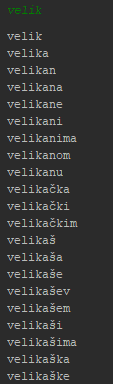
\includegraphics[width=\marginparwidth]{Screenshot_1.png}
\caption{Допуне за реч \textit{велик}}
\label{fig:my_label}
} 

\newpage

\section{Предстaвљање графова у
\\ програмским језицима}
Постоји много начина за репрезентацију графова и сличних структура података у разним програмским језицима. Конкретно, у области такмичарског програмирања, где се жртвује лакоћа коришћења и једноставност зарад ефикасности, се највише користе \textit{матрице суседности} и \textit{листе суседности}. У језицима као што су \textit{Python} или \textit{C\#} постоје или већ уграђене класе, или модули који се врло лако могу искористити. Један од тих модула, \textit{NetworkX} је и коришћен у овом раду за демонстрацију алгоритама за налажење најкраћег пута између два чвора.

\subsection*{Матрица суседности}
Матрица суседности је врло једноставна за имплементацију и коришћење. Правимо матрицу \textbf{M} димензија $V \times V$, где је \textbf{V} број чворова датог графа. За неки елемент $M[i][j] = 1$ постоји ивица између чвора \textit{i} и чвора \textit{j}. Уколико радимо са тежинским графом, користимо $M[i][j] = k$, где \textit{к} представља тежину ивице од чвора \textit{i} до чвора \textit{j}. Матрице суседности треба користити када нам се тражи велик број провера постојања разних ивица, јер се та операција изводи у $\mathcal{O}(1)$. Међутим, због коришћења матрице, коришћење меморије је увек високо, ма колико граф имао ивица. 
\begin{figure}[h]
    \begin{minipage}{0.3\textwidth}
        \centering
    
         \kbordermatrix{
       & 0 & 1 & 2 & 3 & 4 \\
        0 & 0 & 1 & 0 & 0 & 1 \\
        1 & 1 & 0 & 1 & 1 & 1 \\
        2 & 0 & 1 & 0 & 1 & 0 \\
        3 & 0 & 1 & 1 & 0 & 1 \\
        4 & 1 & 1 & 0 & 1 & 0
      }
    \end{minipage}\hfill
    \begin{minipage}{0.6\textwidth}
        \centering
    \begin{tikzpicture}
        \node[shape=circle,draw=black] (x4) at (3,3) {4};
        \node[shape=circle,draw=black] (x3) at (6,3) {3};
        \node[shape=circle,draw=black] (x2) at (9, 4.5) {2};
        \node[shape=circle,draw=black] (x0) at (3,6) {0};
        \node[shape=circle,draw=black] (x1) at (6,6) {1};

        \path[-] (x0) edge (x1);
        \path[-] (x0) edge (x4);
        \path[-] (x4) edge (x3);
        \path[-] (x1) edge (x3);
        \path[-] (x1) edge (x4);
        \path[-] (x1) edge (x2);
        \path[-] (x3) edge (x2);
        
        

    \end{tikzpicture}
    \end{minipage}
    
    \caption{Матрица суседности}
    \label{fig:my_label}
\end{figure}
\subsection*{Листа суседности}
Користимо низ листа или повезаних листта.Сваки елемент низа $G_i$ је листа свих чворова који су суседни \textit{i}-том чвору. Овај начин чувања графа је меморијски веома ефикасан због тога што памти само ивице које постоје, за разлику од матрице суседности. Лоша страна листа суседности јесте спора претрага постојања неке ивице, чија комплексност тежи $\mathcal{O}(V)$, где је \textbf{V} број чворова.

\newpage
\section{Налажење путања}
\subsection{Претрага у дубину (\textit{Depth-first search})}
Претрага у дубину је један од основних алгоритама за претрагу и пролазак кроз граф, чинећи га погодним за решавање графовских проблема и задатака. Креће од кореног чвора у случају стабла или одабраног чвора код осталих врста графова, и иде док може низ сваку	грану, након чега се враћа на последњи избор гранe и бира неку од осталих могућности (тзв. \textit{Backtraking}) 

\subsubsection*{\textbf{Поступак}}
Бирамо почетни чвор \textit{u}, и маркирамо га као посећеног. Позивамо \textit{dfs} за њега. Бирамо једног његовог суседа, чвор \textit{v}, који мора бити непосећен. Маркирамо га и позивамо \textit{dfs} за \textit{v}. Када дођемо до чвора који нема више непосећених суседа или суседа уопште, враћамо се назад на чвор \textit{u}, и бирамо један од његових непосећених суседа. Уколико чвор \textit{u} нема непосећених чворова који су повезани за њега, враћамо се још један корак уназад. Када почетни чвор остане без непосећених суседа, алгоритам је готов.
\begin{figure}[h]
    \centering
    \begin{tikzpicture}[->,>=stealth',every node/.style={circle,draw},level 1/.style={sibling distance=50mm},level 2/.style={sibling distance=20mm},level 3/.style={sibling distance=12mm},
%scale=0.7, transform shape
]
\node (nA){A}
   child { node (nB) {B}
              child { node (nD) {D}
                         child { node (nH) {H} }
                       }
              child {  node (nE) {E}
                         child { node (nI) {I} }
                         child { node (nJ) {J} }
                       }
            }
   child { node (nC) {C}
              child { node (nF) {F}
                         child { node (nK) {K}  }
                         child { node (nL) {L} }
                         child { node (nM) {M} }
                       }
              child {  node (nG) {G} }
             };

  \draw[->,purple,rounded corners,dashed,line width=0.9pt]
    ($(nA) + (-0.4,0.2)$) --
    ($(nB) +(-0.3,0.4)$) --
    ($(nB) +(-0.6,0.0)$) --
    ($(nD)  +(-0.4,0.3)$) --
    ($(nD)  +(-0.5,0.0)$) --
    ($(nH)  +(-0.5,0.0)$) --
    ($(nH)  +(-0.4,-0.35)$) --
    ($(nH)  +(0.0,-0.5)$) --
    ($(nH)  +(0.4,-0.35)$) --
    ($(nH)  +(0.5,0.0)$) --
%    ($(nD)  +(0.45,-0.2)$) --
    ($(nD)  +(0.45,0.0)$) --
    ($(nB)  +(0.0,-0.4)$) --
    ($(nE)  +(-0.45,0.0)$) --
    ($(nI)  +(-0.45,0.0)$) --
    ($(nI)  +(-0.35,-0.35)$) --
    ($(nI)  +(0.0,-0.45)$) --
    ($(nI)  +(0.35,-0.35)$) --
    ($(nI)  +(0.4,0.0)$) --
    ($(nE)  +(0.0,-0.4)$) --
    ($(nJ)  +(-0.45,0.0)$) --
    ($(nJ)  +(-0.35,-0.35)$) --
    ($(nJ)  +(0.0,-0.45)$) --
    ($(nJ)  +(0.35,-0.35)$) --
    ($(nJ)  +(0.45,0.0)$) --
    ($(nE)  +(0.4,0.2)$) --
    ($(nB)  +(0.4,0.0)$) --
    ($(nA)  +(0.0,-0.4)$) --
    ($(nC)  +(-0.4,0.0)$) --
%    ($(nF)  +(-0.6,0.0)$) --
    ($(nK)  +(-0.5,0.1)$) --
    ($(nK)  +(-0.4,-0.35)$) --
    ($(nK)  +(0.0,-0.5)$) --
    ($(nK)  +(0.4,-0.3)$) --
    ($(nF)  +(-0.15,-0.4)$) --
    ($(nL)  +(-0.5,0.0)$) --
    ($(nL)  +(-0.4,-0.35)$) --
    ($(nL)  +(0.0,-0.5)$) --
    ($(nL)  +(0.4,-0.35)$) --
    ($(nL)  +(0.5,0.0)$) --
    ($(nF)  +(0.15,-0.4)$) --
    ($(nM)  +(-0.5,0.0)$) --
    ($(nM)  +(-0.4,-0.35)$) --
    ($(nM)  +(0.0,-0.5)$) --
    ($(nM)  +(0.4,-0.35)$) --
    ($(nM)  +(0.5,0.2)$) --
    ($(nF)  +(0.4,0.0)$) --
    ($(nC)  +(0.0,-0.4)$) --
    ($(nG)  +(-0.5,0.0)$) --
    ($(nG)  +(-0.4,-0.35)$) --
    ($(nG)  +(0.0,-0.5)$) --
    ($(nG)  +(0.4,-0.35)$) --
    ($(nG)  +(0.5,0.1)$) --
    ($(nC) +(0.6,0.0)$) --
    ($(nC) +(0.3,0.4)$) --
    ($(nA) + (0.4,0.2)$);
\end{tikzpicture}
    \caption{Пролазак кроз граф дубински}
    \label{fig:my_label}
\end{figure}
\subsubsection*{Пример коршићења дубинске претраге}
Претрагу у дубину можемо користити за небројено много ствари. Једна од њих је налажење циклуса у графу. Сам алгоритам је врло једноставан. Крећемо се кроз граф, и наилазимо на чвор $v$. Ако чвор $v$ има суседа $u$, тако да је $u$ већ посећен, нити је родитељ чвора $v$, тада граф садржи циклус.\par
Исто тако, дубинску претрагу можемо да користимо да видимо да ли је граф бипартидан. Почетни чвор поставимо на једну од две боје. Према правилима бипартидности, тада његово дете мора бити друге боје. Ако на овај начин успемо да попунимо, односно обојимо, цео граф, онда је он бипартидан.

\subsection{Претрага у ширину (\textit{Breadth-first search})}
Као и претрага у дубину, и претрага у ширину је један од базичних алгоритама за пролазак кроз граф. Такође бирамо чвор од кога крећемо или у случају стабла, корен. Разлика је у томе што \textit{bfs} прво проверава све суседе једног чвора пре него што настави низ граф. 
\subsection*{Поступак}
\begin{enumerate}
    \item Бирамо чвор \textit{u}, и маркирамо га као посећеног. 
    \item Прођемо кроз све његове суседе, и оне који нису посећени додамо у \textit{ред} непосећених
    \item Избацити тренутни чвор, и изабрати следећи у \textit{реду}
\end{enumerate}
Ове кораке треба понављати све док сви чворови нису маркирани.
\subsubsection*{Пример коришћења претраге у ширину}
\setlength{\epigraphwidth}{0.75\textwidth}
\epigraph{\textit{Дата су два броја, $n$ и $m$. Циљ је трансформисати $n$ у $m$, користећи две операције: множење са два или смањивање за један. Тражи се минималан број операција.}}{Задатак 520B са сајта \textit{Codeforces}}
Временско ограничење овог задатка је $2s$, а просторно $256 MB$. И $n$ и $m$ испуњавају $1 \leqslant n, m \leqslant 10^4$. \par
Конструисаћемо граф где су чворови бројеви, а ивице између два чвора знак да једном операцијом први број можемо претворити у други. Такође, уочавамо да нема потребе за чворовима чији је број већи од $2m$, тако да ћемо у најгорем случају имати $2 \cdot 10^4$ чворова и $4 \cdot 10^4$ ивица, што значи да је претрага у ширину довољно ефикасна за брзо решавање проблема. \par Крећемо од чвора са бројем $n$. Пролазимо кроз све његове суседе, и гледамо да ли је неки од њих тражени број. Уколико се број $m$ не налази међу њима, гледамо суседе суседа, све док не наиђемо оно што желимо. Поставља се питање зашто овде користимо претрагу у ширину, а не дубинску претрагу. Проблем гледања у дубину јесте што, први пут када наиђемо на $m$, то не мора да значи да је број ивица до тада минималан, што није случај са претрагом у ширину. Када гледамо \glqq слојевито \grqq, сви суседи су у истом нивоу, односно број корака до њих је исти, минималан. \par У овом примеру, начин имплементирања графа не утиче много на крајњи резултат. Комплексност за матрицу суседности је $\mathcal{O}(V^2)$, где је \textbf{V} број чворова, а за листу суседности $\mathcal{O}(|V| + |E|)$, где је \textbf{E} број ивица.

\subsection{Налажење најкраће путање}
\subsubsection*{Флојд-Варшалов (\textit{Floyd–Warshall}) алгоритам}
Флојд-Варшалов алгоритам налази најкраћу дужину пута измеу свака два чвора у графу. Иако сам по себи не враћа најкраћу руту од чвора А до чвора Б, можемо је извући тако што извршимо малу модификацију у коду. Овај метод је класичан пример динамичког програмирања. Комплексност овог алгоритма је $\Theta(V^3)$, где је \textit{V} број чворова. Слабост Флојд-Варшала је у томе што не ради са графовима у којима постоје \textit{негативни циклуси}. Негативни циклус је циклус чворова чија је сума ивица мања од 0. \par
Флојд-Варшал, иако не баш ефикасан, се често појављује на разним такмичењима из програмирања. Иако је спор, имплементира се веома брзо, и идеалан је за графове са мало чворова.

\subsubsection*{Дајкстрин (\textit{Dijkstra}) алгоритам}
Дајкстрин алгоритам је један од најпознатијих и најкоришћенијих алгоритама који је нашао своју употребу у најразличитијим областима. Предложен је 1959. године у раду \textbf{Едсгера Дајкстре}, холандског информатичара\footnote{’A Note on Two Problems in Connexion with Graphs’, Numerische Mathematik 1959}. Најчешћа примена овог алгоритма јесте тражење најкраћег пута између два специфична чвора неког тежинског графа (\textit{Single source shortest path}). Алгоритам можемо поделити на шест корака, претпостављајући да хоћемо да нађемо најкраћи пут од чвора $X_0$ до чвора $X_n$:
\begin{enumerate}
    \item Направити сет непосећених чворова и маркирати све чворове као \textit{непосећене}.
    \item Поставити \textit{привремену} тежину почетног чвора на нулу, $w(X_0) = 0$. Затим, ставити  \textit{привремену} тежину свих осталих чворова на бесконачно, $w(X_i)=\infty$ за сваки чвор \textit{$X_i$}.
    \item Претражити све непосећене суседе тренутног чвора и изабрати чвор са најмањом \textit{привременом} тежином. \textit{Привремена} тежина се рачуна као збир тежине ивице између та два чвора и \textit{привремене} тежине полазног чвора.\\
    \begin{center}
            $w(X_{i+1}) = w(X_{i}) + E_{i, i+1}$  
    \end{center}
    Ако је тренутна вредност \textit{привремене} тежине чвора $X_i$ мања од новоизрачунате, $w(X_i)$ остаје непромењен.
    \item Након разматрања свих суседа, маркирамо чвор као посећен и избацаујемо га из сета непосећених. Једном посећен чвор се не може опет узети у обзир.
    \item Ако је циљани чвор посећен, или је најмања вредност у скупу \textit{привремених} тежина једнак бесконачности (не постоји веза између два чвора за које тражимо најкраћи пут), алгоритам се зауставља.
    \item У другом случају, изабрати чвор са најмањом \textit{тренутном} тежином као нови тренутни чвор и вратити се на корак број 3.

\end{enumerate}
Дајкстрин алгоритам се већински користи у развоју и употреби мрежа путева, а један је и од подпротокола за рутирање пакета. Сложеност зависи од начина примене. Дајкстрин првобитни алгоритам ради у временској сложености од $\mathcal{O}(|V|^2)$, где је \textbf{V} број чворова. Даљим унапређивањем путем коришћења \textit{реда} са приоритетомо имплементираног путем \textit{Фибоначијевог хипа}  (\textbf{Fibonacci heap}) комплексност је снижена на $\mathcal{O}(|E| + |V|log|V|)$, где је \textbf{Е} број ивица.
\subsubsection*{Коришћење Дајкстриног алгоритма за решавање лавирината}
За израду примера и слика коришћен је \textit{Python 3.5}, са модулима \textbf{NetworkX} за лакши рад са графовима и \textbf{matplotlib} за скицирање и израду решења. Од додатног софтвера, коришћен је \textit{Daedalus} за генерисање лавирината. \par
Полазна идеја је да треба решити $N\times N$ лавиринт, где је \textbf{N} број редова односно колона. Сваки пиксел можже бити или бео или црн. Бео пиксел означава простор за кретање, док је црни ознака за зид. Овај задатак може се решити из 5 стадијума.
\begin{enumerate}
    \item Скенирати слику и направити мапу слике у меморији. Ако је пиксел црн, односно бео, запамтити га као таквог.
    \item Бирање чворова.
    \begin{itemize}
        \item Ако је тренутни пиксел проходан и има бар 3 различите стране на које може да крене, такав пиксел постаје чвор.
        \item У супротном, пиксел не постаје чвор и као такав касније постаје део ивице.
    \end{itemize}
    \item Итеративни пролазак кроз мапу пиксела и рачунање тежина ивица. 
    \item Примена Дајкстриног алгоритма на новонастали граф.
    \item Цртање и чување решеног лавиринта.
    
\end{enumerate}
\begin{figure}
    \begin{minipage}{0.5\textwidth}

        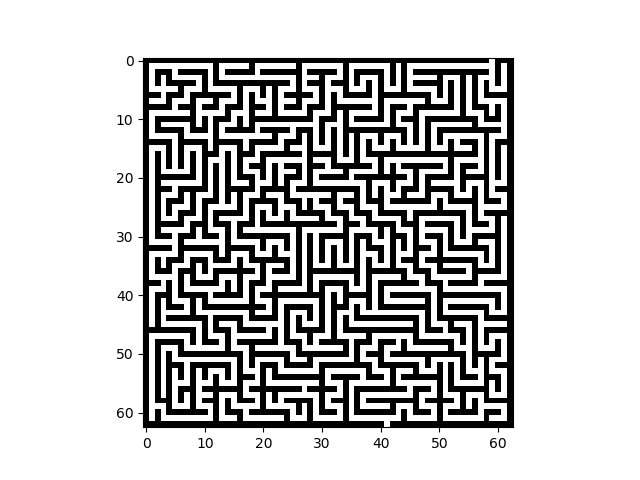
\includegraphics[scale=0.4, left]{baza.png}
        \caption{$64\times 64$ лавиринт}
        \label{fig:my_label}
    \end{minipage}
    \begin{minipage}{0.5\textwidth}
        \centering
        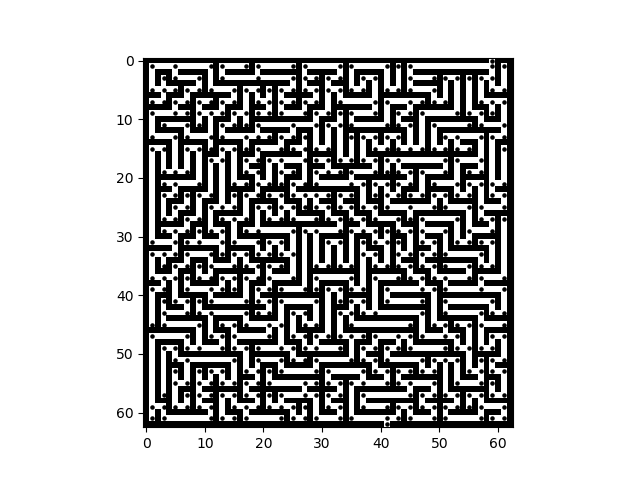
\includegraphics[scale=0.6, left]{tacke.png}
        \caption{Чворови}
        \label{fig:my_label}
    \end{minipage}
\end{figure}
\begin{figure}
    \begin{minipage}{0.5\textwidth}
    \centering
        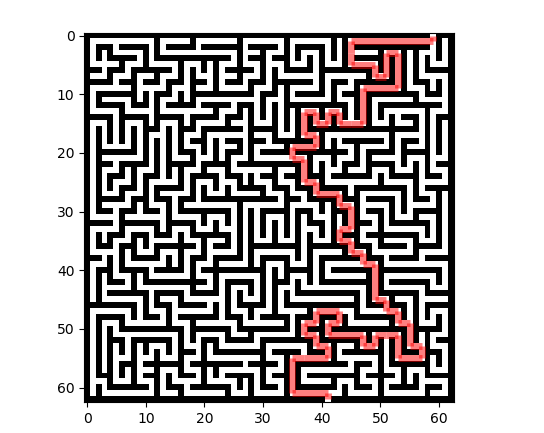
\includegraphics[scale=0.4, left]{64.png}
        \caption{Решен лавиринт}
        \label{fig:my_label}
    \end{minipage}
    \begin{minipage}{0.5\textwidth}
    \centering
        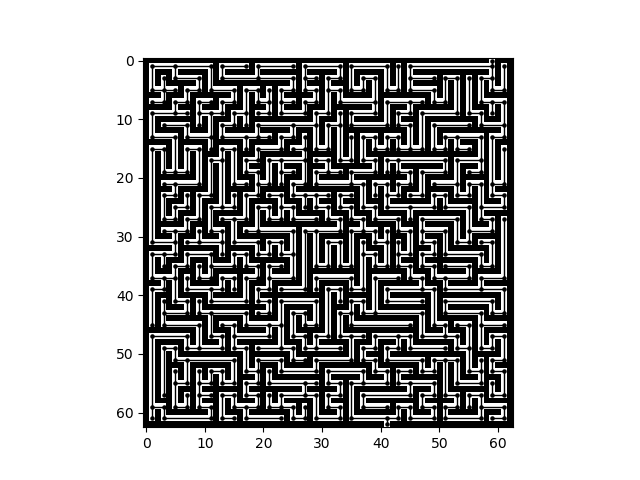
\includegraphics[scale=0.6, left]{linije.png}
        \caption{Ивице}
        \label{fig:my_label}
    \end{minipage}
    
\end{figure}


\subsubsection*{Форд-Белманов (\textit{Bellman–Ford}) алгоритам}
Форд-Белманов алгоритам тражи најкраћу путању од задатог чвора до свих осталих чворова. Користи се као алтернатива Дајкстрином алгоритму због тога што, иако временски спорија, може да ради са тежинским графовима који имају негативне ивице. Још једна специфична употреба овог метода јесте детекција негативних циклуса. У том случају не постоји пут са најмањом тежином јер је увек могуће проћи још једном кроз циклус и смањити тежину.

\par
Овај алгоритам примењује одређене принципе динамичког програмирања, у томе да рачуна најкраће удаљености одоздо на горе. Прво рачуна најкраће путеве за највише једну ивицу, па најкраће путеве за највише две ивице и тако све до најкраћег пута са $|V|-1$ ивица, где је \textbf{V} број чворова. Због тога је комплексност Форд-Белмана $\mathcal{O}(|E| \cdot |V|)$, где је \textbf{E} број ивица, а \textbf{V} број чворова.
\subsubsection*{А* алгоритам}
А* (А-звезда) алгоритам је један од најраширенијих и најефикаснијих алгоритама за тражење најкраће путање између два чвора. Оно што издваја овај алгоритам од осталих јесте што користи хеуристичке методе за процену најбољег чвора. Хеуристику, једноставним језиком, можемо назвати \glqq паметним погађањем\grqq. На пример, пре покретања алгоритма бисмо израчунали удаљеност свака два чвора. Неке од честих хеуристичких функција које користимо јесу \textit{Менхетн дистанца}, \textit{Еуклидска дистанца}, или чак \textit{дијагонална дистанца}. Циљ алгоритма је да минимизује
\begin{center}
    $f(n) = g(n) + h(n)$,
\end{center}
где је $n$ следећи чвор који се бира, $g(n)$ цена путање од почетка до сада, а $h(n)$ вредност хеуристичке функције. У случају да је $h(n) = 0$ за сваки чвор, алгориттам се своди на Дајкстрин. \par
Комплексност А* алгоритма у великом проценту зависи од хеуристичкке функције, а и самог графа. У неким случајевима, сложеност може пасти и на полиномно време. Један од великих проблема оваквог тражења најкраћег пута јесте избор саме хеуристичке функције. Лоше изабрана функција може донети неоптималне, односно нетачне резултате. Сам алгоритам решава чест проблем тражења путања у видео играма, иако је првобитно био дизајниран специфично за графове.

\section{Минимално стабло разапињања \\
(\textit{Minimum spanning tree})}
Минимално стабло разапињања је скуп ивица повезаног тежинског графа такав да су сви чворови повезани без циклуса и чија је сума ивица најмања могућа. Потреба за оваквим стаблима потиче из потраге за ефикасним начином постављања електричне мреже на неком простору. Минамална стабла разапињања своју примену, између осталог налазе и у телекомуникацијским и компјутерским мрежама, водоводним мрежама, таксономији\ldots \par
Минимална стабла разапињања се најчешће траже Примовим или Крускаловим алгоритмом.
\begin{figure}[ht]
    \centering
    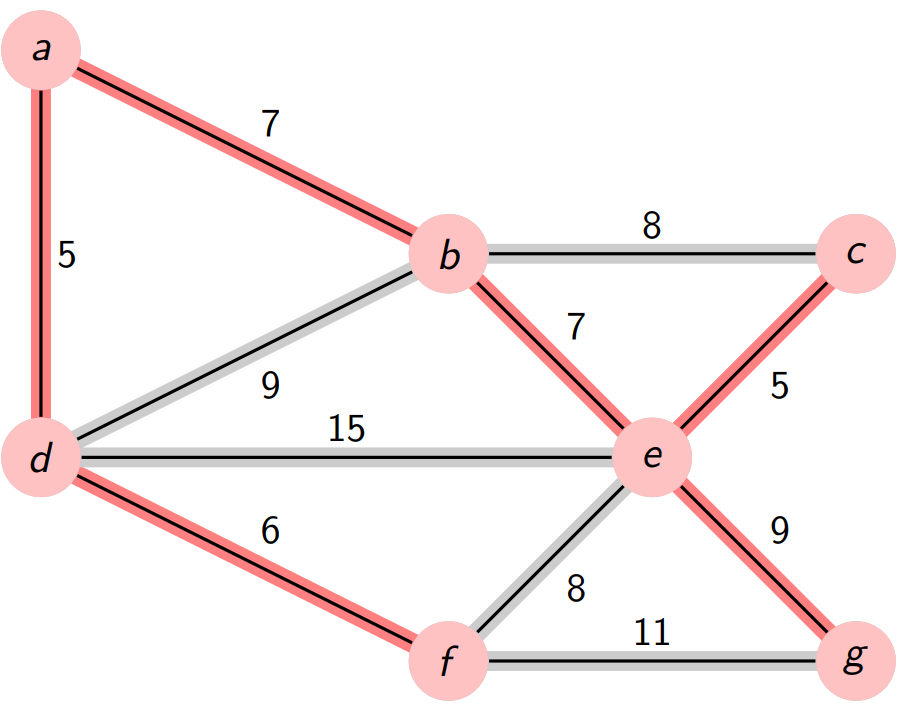
\includegraphics[scale=0.5]{primn.png}
    \caption{Минимално стабло разапињања}
    \label{fig:my_label}
\end{figure}
\newpage
\subsection{Примов алгоритам}
Примов алгоритам је \textit{грамзиви} алгоритам који одређује минимално стабло разапињања. Поприлично је једноставан и може се поделити на четири корака: 
\begin{enumerate}
    \item Изабрати почетни чвор
    \item Проћи кроз све чворове који су повезани са чворовима у тренутном стаблу и нису у самом стаблу
    \item Изабрати чвор који има најмању тежину и повезати га са стаблом
    \item Вратити се на корак 2 све док не останемо без чворова
\end{enumerate}
Комплексност Примовог алгоритма у његовом основном облику при коме га имплементирамо преко матрице суседности има износи $\mathcal{O}(|V|^2)$, где је \textbf{V} број чворова. Као и Дајкстрин, и Примов алгоритам се може значајно убрзати коришћењем Фибоначијевог хипа. Тада је комплексност $\mathcal{O}(|E| + |V|log|V|)$, где је \textbf{E} број ивица. Такође, Примов алгоритам има потенцијал да се користи паралелно, што може довести до великог унапређења у брзини извршавања. 
\subsection{Крускалов алгоритам}
Крускалов алгоритам је такође \textit{грамзив} алгоритам, али његова комплексност је $\mathcal{O}(|E| log|E|)$, где је \textbf{Е} број ивица.
Једна од основних примена структуре података која се зове дисјунктни-сет јесте у Крускаловом алгоритму. 
\begin{enumerate}
    \item Направити \textit{шуму} (скуп стабала) где је сваки чвор засебно стабло
    \item Направити скуп свих ивица
    \item Све док је скуп ивица непразан и шума непразна
    \begin{itemize}
        \item Узети ивицу најмање вредности из скупа ивица
        \item Ако та ивица повезује два стабла, додати је у шуму
    \end{itemize}
    
\end{enumerate}

\subsubsection*{Пример коришћења Крускаловог алгоритма}
Често су проблеми који захтевају минимално стабло разапињања записани тако да се на први поглед не примећује да задатак захтева тражење МСР-а. Један такав задатак јесте задатак \glqq Трке\grqq\footnote{Задатак 1234 са UVa платформе}. Дат нам је план града (раскрснице су чворови, а улице ивице). Циљ задатка је да се поставе камере на све циклусе, да би се спречиле илегалне трке, а да цена камера буде минимална. Цена камера се рачуна као збир тежина ивица на које су постављене камере.\par
Поента овог задатка је приметити да су ивице које не припадају \textit{максималном} стаблу разапињања (понаша се и тражи исто као и минимално, само се тражи највећи могући збир) идеалне позиције за постављање камера. Разлог коришћења МСР у овом примеру јесте то што МСР налази стабло без циклуса. Свака ивица која не припада максималном стаблу разапињања је део неког циклуса, односно неке трке коју треба да уочимо. Због тога што смо тражили максимално стабло, знамо да су цене тих ивица најмање могуће, па је и решење минимално.  \par
Креираћемо шуму чворова где је један чвор шума за себе. Сортирамо скуп ивица који смо креирали приликом уноса података нерастући (тражимо максимално стабло разапињања). Итерирамо редом кроз сортиране ивице, и помоћу дисјунктног сета проверавамо да ли су два чвора повезана том ивицом део истог стабла. Ако нису, повежемо их и усмеравамо пажњу на следећу ивицу. Ако јесу, на коначно решење додајемо тежину те ивице. Када остане без ивица, алгоритам прекида са радом.
\newpage

\section{Бојење графова}
Бојење је један од специјалних начина обележавања графа. У основи, може се објаснити на једноставан начин: обојити сваки чвор неком бојом тако да ниједан његов сусед није обојен том истом бојом. Осим класичног бојења чворова, постоје и проблеми бојења ивица, као и проблеми бојења површина који се могу трансформисати у проблем бојења чворова. \par
Овакав тип проблема се често јавља у природи, па је и сама област бојења графова изразито развијена. Неке од најпознатијих примена јесу:
\begin{itemize}
    \item Планирање распореда и редова вожње
    \item Распоређивање фреквенција разним антенама и радио торњевима
    \item Бојење мапа
    \item Проверавање бипартидности графа
    \item Решавање судокуа
\end{itemize}
\textit{Хроматским бројем} називамо минимални број боја довољан да обојимо граф. Специјални случај јесте да \textit{хроматски број} износи два. Тада је граф бипартидан. 


\subsection{Теорема о четири боје}
\epigraph{\textit{Може ли се билло која карта обојити користећи највише чеитири боје тако да суседне државе буду различито обојене}?}{}

Прву поставку овог проблема саставио је француски математичар \textbf{Френсис Готрије} 1852. године, када је покушао да обоји мапу Енглеске.\footnote{Donald MacKenzie, Mechanizing Proof: Computing, Risk, and Trust (MIT Press, 2004) стр. 103} Приметио је да је за испуњавање целе мапе потребно само четири боје. Ова теорема, наоко лака за доказивање, мучила је математичаре све до 1976. године, када су је Волфганг Хакен и Кенет Апел доказали 
користећи рачунар за доказ. Теорема о четири боје је прва већа теорема доказана коришћењем рачунара, и због тога сам рад није био прихваћен од стране свих математичара јер није могуће проверити све податке ручно. Двадесет и једну годину касније, објављен је једноставнији доказ који користи сличне идеје који је ставио тачку на већину дискусија.

\begin{figure}

    \centering
    
\includegraphics[scale=0.6]{download.png}
    \caption{Пример површине обојене користећи тачно 4 боје\footnotemark }
    \label{fig:my_label}

    
\end{figure}

\newpage
\section{Проблем путујућег трговца \\
 (\textit{Travelling salesman problem})}
\setlength{\epigraphwidth}{0.85\textwidth}

\epigraph{
\textit{Претпоставимо да трговачки путник жели да обиђе известан број градова. Којим редоследом трговачки путник треба да обилази градове, тако да сваки град обиђе једанпут, да се по обиласку свих градова врати у почетни град и да при томе пређе најмање могуће растојање?}
 }{}
 
Проблем путујућег трговца је један од класичних и најпознатијих алгоритамских проблема. Фокусиран је на \textit{оптимизацију}, односно тражење бржег, краћег и јефтинијег решења. \par
\footnotetext{Генерисано помоћу https://github.com/akleemans/fourcolors}
Порекло ППТ још увек није сасвим разјашњено. Први пут се појављује још 1832. године у трговачком приручнику, али без икакве математичке подлоге\footnotemark. Први математичари који су обратили пажњу на овај проблем јесу В.Р. Хамилтон и Томас Киркмен, који су га тада назвали \textit{Поштарев проблем}. Оно што је ставило ППТ у први план јесте стандардизовање $P = NP$ проблема и његово уврштање у \textit{Миленијумске проблеме}, који ономе ко га реши обезбеђује награду од милион долара.
\footnotetext{\textit{Der Handlungsreisende wie er sein soll und was er zu thun hat, um Aufträge zu erhalten und eines glücklichen Erfolgs in seinen Geschäften gewiß zu sein ; Mit e. Titelkupf. / von einem alten Commis-Voyageur}}

\par
Најдиректније и најочигледније решење јесте да се нађе најбоља опција од свих могућих пермутација (тзв. \textit{brute-force}). Међутим, овакав приступ тежи комплексности од $\mathcal{O}(n!)$, што постаје непрактично за више од 20 градова.\par
Једна од првих примена динамичког програмирања јесте Хелд-Карпов алгоритам из 1962. године, који је смањио комплексност на $\mathcal{O}(n^2 2^n)$.
\subsection*{}
Поред директних алгоритама постоје и разни хеуристички и алгоритми за апроксимацију који могу ефективно и у великом степену прецизно проценити најбољи пут. \par
\textit{Алгоритам најближег комшије} је грамзиви алгоритам бира најближи непосећени град као следећи корак. Овај метод брзо даје ефективан и кратак пут. У просеку, пут изабран на овај начин је око 25\% дужи од најкраћег могуће руте. Процена је да овај алгоритам има комплексност $\Theta(log|n|)$ за све комбинације које испуњавају неједнакост троугла.\par
\textit{Кристофајдсов алгоритам} је апроксимативни алгоритам који користећи минимално стабло разапињања успева да одреди пут који је максимално 1,5 пута већи од идеалне руте. До сада, овај метод има најмањи \textit{апроксимативни однос}. \par
Са напретком на пољу вештачке интелигенције и машинског учења осмишљена су и неки другачији методи који користе \textit{Марков ланце} и симулације мрављих колонија.
\newpage
\section{Закључак} 
Јасно је да су графови и њихова примена у данашњем свету изузетно битни, и зато је важно разумети како они функционишу и како радити са њима.\par
Суштина овог рада јесте да, коришћењем једноставних примера и објашњења, уведе читаоца у свет теорије графова. Иако је та област математике и програмирања много дубља, опширнија и компликованија од онога што је у овом раду покривено, велик број урађених алгоритама може решити свакодневне проблеме са којима ће се читалац сусрести, као што је програмирање мрежа и преноса података, рад са базама података и друго. Такође, алгоритми који су овде обрађени су добра подлога за даљи рад и учење, и имају изузетно много примена у најразличитијим областима. Два историјска проблема покривена на крају рада, \textit{Теорема о четири боје} и \textit{Проблем путујућег трговца}, су пример тога колико ће се људи жртвовати зарад напретка науке и бољег сутра.

\newpage
\section{Референце}
\renewcommand{\section}[2]{}
\begin{thebibliography}{6}
\bibitem{CP3}
Steven Halim, Felix Halim. \textit{Competitive Programming 3}, 2013.
\bibitem{CP}
Antti Laaksonen. \textit{Competitive Programming Handbook}, 2017.
\bibitem{Boje}
Donald MacKenzie.\textit{Mechanizing Proof: Computing, Risk, and Trust} MIT Press, 2004.
\bibitem{Dijkstra}
Edsgar Dijkstra, \textit{A note on Two Problems in Connexion with Graphs}, Numerische Mathematik, 1959.
\bibitem{CodeF}
https://codeforces.com
\bibitem{UVa}
https://uva.onlinejudge.org/index.php
\bibitem{git}
https://github.com/akleemans/fourcolors

\end{thebibliography}





























\end{document}
